\chapter{Modèle de l'apprenant et découverte des prérequis} 
\minitoc
\thispagestyle{empty}
\newpage
\section{Introduction}
Le terme "apprentissage" fait souvent référence à l'apprentissage électronique ou e-learning. L’apprentissage en ligne, l'apprentissage à distance et l'apprentissage en ligne. L'apprentissage en ligne est connu comme des activités d'étude avec le soutien d'un ordinateur et d'un réseau (Fröschl, 2005, p. 12). \\
Dans l'apprentissage en ligne, la communication entre les apprenants et les enseignants ou les apprenants et les apprenants se fait sur le réseau ou sur Internet, les supports d'apprentissage sont souvent des documents électroniques tels que des pages Web et des fichiers au lieu de livres traditionnels sur papier \cite{learner_model__adaptive_learning}. Dans ce chapitre, nous décrivons la modélisation de l'apprenant compte tenu de son importance dans tous les domaines de recherche. Nous commençons par une présentation des notions du modèle de l'apprenant et des caractéristiques des méthodes utilisées pour la modélisation de l'apprenant. Puis nous terminons avec la Découverte des prérequis.

\section{Learner Model}

\subsection{Définition}
Winkels décrit le modèle de l'apprenant comme une structure de données qui reflète l'état des connaissances supposées de l'apprenant sur un domaine cible (le domaine d'apprentissage) \cite{user_modelling_help_systems}. Selon Self, le modèle de l'apprenant devrait inclure les informations suivantes : les connaissances et les idées fausses de l'apprenant, ses compétences et son comportement. Pour déterminer ce que l’apprenant a fait, Self souligne qu’il est nécessaire d’avoir un historique des interactions de l’apprenant avec le système \cite{user_learner_modeling_workbench}. \\
Greer considère le modèle de l'apprenant comme une représentation abstraite des croyances, des connaissances et des compétences de l'apprenant dans le système, y compris l'historique des actions de l'apprenant qui peut être analysé et interprété \cite{psycho_oncology}.

\subsection{Caractéristiques des méthodes utilisées pour la modélisation de l'apprenant}
Il existe plusieurs modèles existants classés selon la nature des informations extraites par le modèle et les méthodes utilisées pour les traiter \ref{Caracteristiques_modelisation_apprenants1} et \ref{Caracteristiques_modelisation_apprenants2}. \cite{student_model_centered_architecture}

\begin{table}[H]
	\centering
	\addtolength{\leftskip} {-4cm}
	\addtolength{\rightskip}{-4.5cm}
	\begin{tabular}{|m{3cm}|m{5cm}|m{5cm}|m{4cm}|}
	\hline
	\rowcolor{blueforest}
	\color{white} \textbf{Méthodes} & \color{white} \textbf{Applications} & \color{white} \textbf{Avantage} & \color{white} \textbf{Limites} \\
	\hline\hline
	\textbf{Modèle de superposition} \newline {------------------} \newline  \textbf{Modèle différentiel}   &
	  Modélisation des connaissances  de l'apprenant à travers   le modèle de connaissance. \newline {-------------------------------} \newline  Identification des lacunes dans les connaissances des apprenants &
	  -Haute expressivité des   problèmes complexes et   flexibilité du raisonnement humain.\newline - utilisation de la structure   du modèle de connaissance.&
	  -Impossible de détecter   les erreurs de l'apprenant \newline -La complexité dépend de   la structure du domaine. \newline  - Défaut de modéliser   les erreurs de l'apprenant. \\ \hline
	  \textbf{Modèle d'erreur}  &
	  Identification des erreurs et fausses croyances de l'apprenant sur un domaine.&
	  Identification des erreurs et fausses croyances de l'apprenant dans un domaine.&
	  Difficulté à modéliser et à définir les erreurs. \\ \hline
	  \textbf{Stéréotypes}  &
	  Classification des apprenants selon des caractéristiques communes, les plus utilisées sont : le style d'apprentissage, le style cognitif, le niveau de connaissance et les préférences.&
	  Initialisation de nouveau caractéristiques de l'apprenant. & \\ \hline
	  \textbf{Les ontologies}  &
	  -Modélisation du modèle de connaissance. \newline
	  -Réutilisation et partage des ressources.&
	  -Ajout de sémantique aux relations entre concepts. \newline
	  -Réutilisation des ressources.&  \\ \hline
	  \textbf{Logique floue}  &
	  -Expression linguistique du niveau de connaissance. \newline
	  -Évaluation des apprenants.\newline
	  -Identification du style de l'apprenant.&
	  -Expression du degré d'incertitude. \newline
	  -Grande expressivité linguistique et logique.&
	  -Consommation de ressources \newline
	  -Pas d'apprentissage. \\ \hline
	\end{tabular}
	\caption{Caractéristiques des méthodes utilisées pour la modélisation des apprenants partie[1]}
	\label{Caracteristiques_modelisation_apprenants1}
\end{table}

\begin{table}[H]
	\centering
	\addtolength{\leftskip} {-4.5cm}
	\addtolength{\rightskip}{-4cm}
	\begin{tabular}{|m{3cm}|m{5cm}|m{5cm}|m{4cm}|}
	\hline
	\rowcolor{blueforest}
	\color{white} \textbf{Méthodes} & \color{white} \textbf{Applications} & \color{white} \textbf{Avantage} & \color{white} \textbf{Limites} \\
	\hline\hline
	  \textbf{Réseau Bayésien}  &
	  -Apprendre et prédire le comportement et le raisonnement de l'apprenant. \newline
	  -Classement des apprenants. \newline
	  -Prédiction des performances des apprenants.&
	  -Apprendre et s'adapter à un environnement incertain.\newline
	  -Résoudre le problème « onlearning » \newline
	  -Fonction avec des données manquantes.&
	  -Consommation de ressources \newline
	  -Difficulté à comprendre les inférences (interprétation) \newline
	  -Grand nombre de variables utilisées. \\ \hline
	  \textbf{Programmation génétique}  &
	  - Recommandation d'un chemin de navigation optimal. \newline
	  -Prédiction des performances des apprenants. \newline
	  -Amélioration des algorithmes de classification.&
	  -Recherche globale \newline
	  -représentation flexible aux changements. \newline
	  -des recherches puissantes dans un espace de problèmes complexes et mal définis.&
	  -Temps d'exécution \newline
	  -Convergence vers les optima locaux \\ \hline
	  \textbf{Réseau flou de neurones}  &
	  -Évaluation et prédiction des performances des apprenants.&
	  -Grand Expressivement \newline
	  -Apprentissage \newline
	  -gestion des incertitudes.&
	  La complexité augmente avec le nombre d'entrées du réseau. \\ \hline
	\end{tabular}
	\caption{Caractéristiques des méthodes utilisées pour la modélisation des apprenants partie[2]}
	\label{Caracteristiques_modelisation_apprenants2}
\end{table}

\subsection{Composantes du modèle de l'apprenant}
\begin{figure}[H]
	\begin{center}
		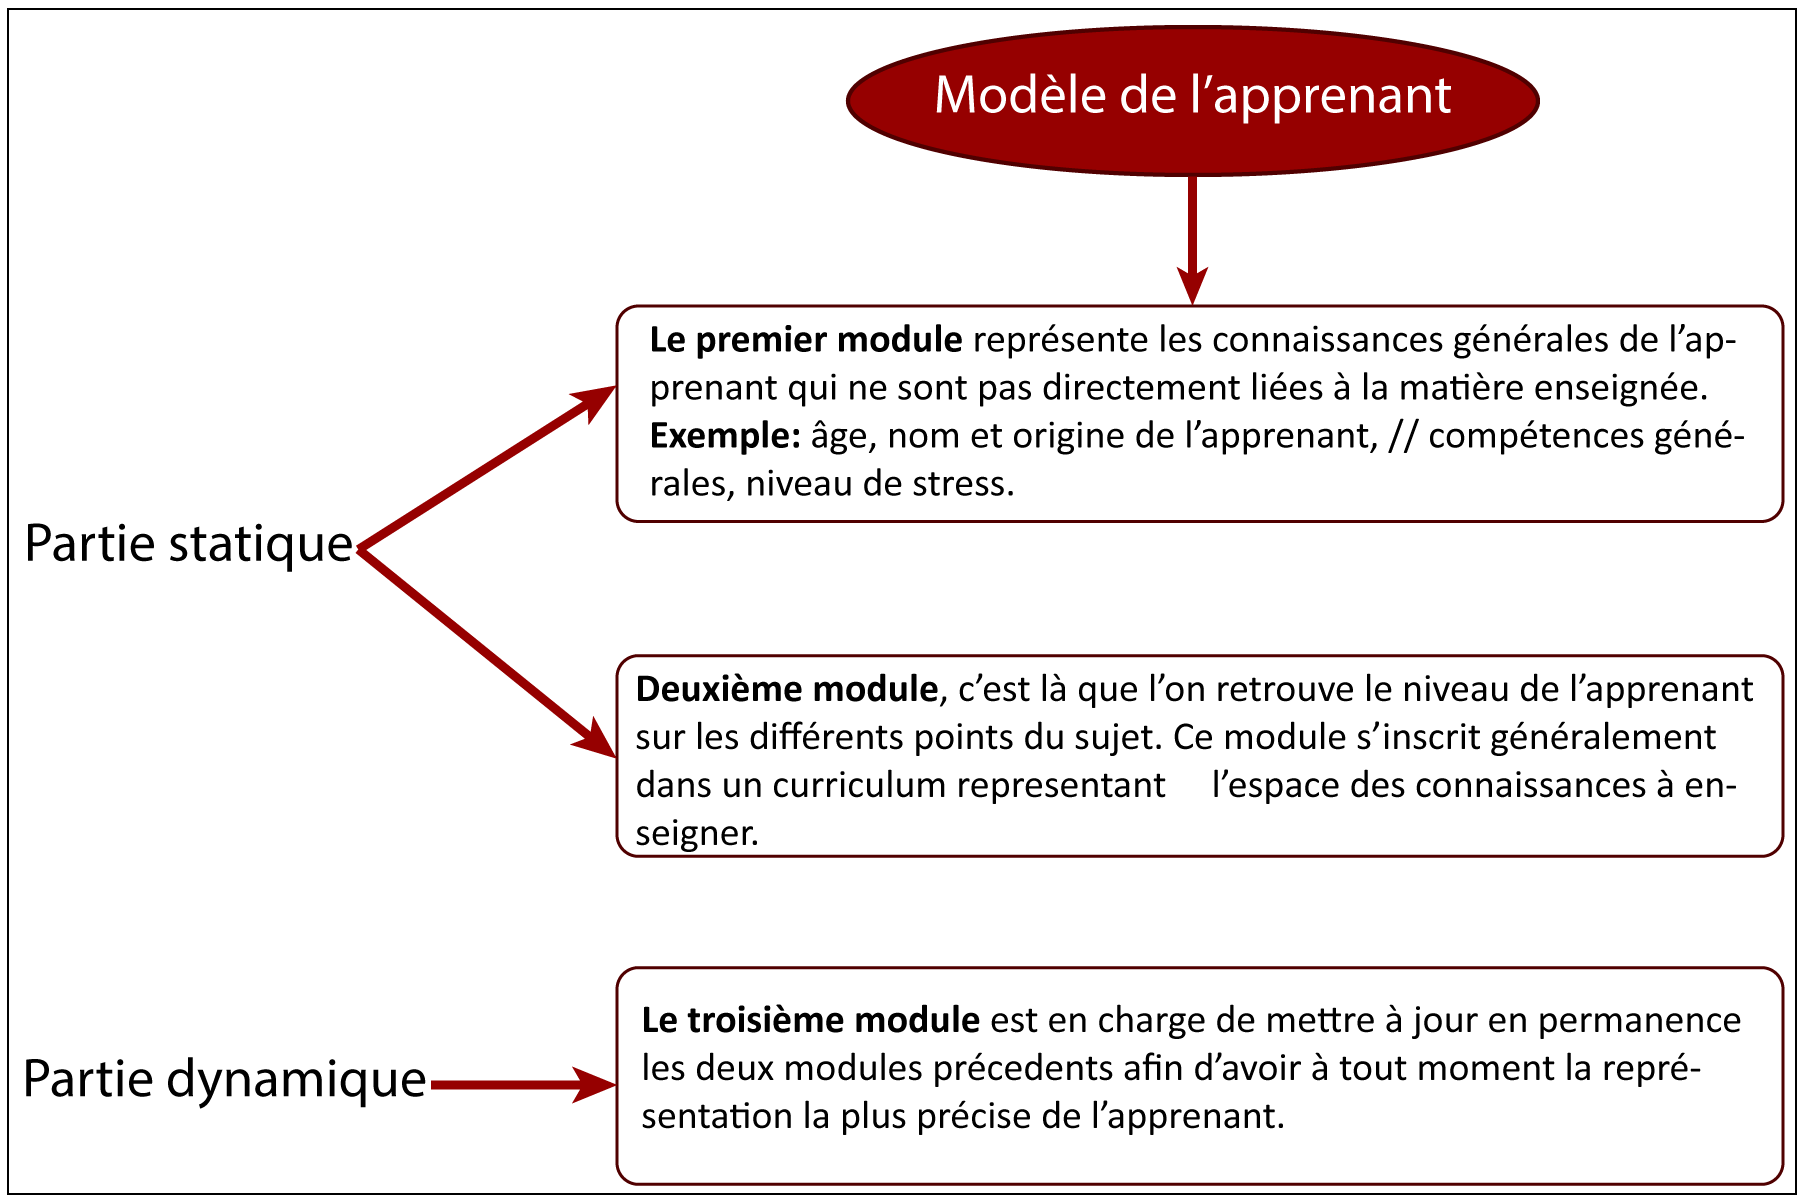
\includegraphics[width=\textwidth]{images/chapitre2/Composante_modele_apprenant.png}
	\end{center}
\caption{Composantes du modèle de l'apprenant}
\label{learnerModel}
\end{figure}
Carr et Goldstein citent, par exemple, quatre informations nécessaires pour maintenir ce modèle : la difficulté du sujet, les questions directement posées par l’apprenant, la performance de l’apprenant et son expérience d’apprentissage \cite{knowledge_based_scheduling_program}. Self définit le modèle de l'apprenant comme un 4-tuplet contenant les variables P (connaissance procédurale), C (connaissance conceptuelle), T (caractéristiques individuelles) et H (histoire) \cite{Elster1987self}. \\
Un modèle de l'apprenant \ref{learnerModel} comprend toujours des connaissances liées au domaine d'enseignement : ce que l'apprenant sait et ce que l'apprenant peut faire. Dans son état le plus complet, ce modèle comprend également des connaissances indépendantes du domaine enseigné. Certaines de ces connaissances sont liées à ses mécanismes d'apprentissage : comment fonctionne l'apprenant ? Comment découvre-t-il de nouveaux concepts ? De nouvelles techniques ? Etc. Les autres concernent les stratégies pédagogiques correspondantes : quels sont les types et modalités d'intervention les plus efficaces ? Etc. \\
Selon Nkambou, le modèle de l'apprenant est identifié en trois parties: \cite{modeles_outils_applications}

\subsubsection{Modèle cognitif}
Description de l’état des connaissances de l’apprenant par rapport au sujet considéré par le bailleur de fonds. Ces informations concernent :
\begin{itemize}
	\item[$\bullet$] \textbf{Capacités :} les informations sur les capacités reflètent le niveau de connaissances de l'apprenant. Robert M. Gagne a classé les capacités de l’apprenant en cinq catégories : l’information verbale, les compétences intellectuelles, les attitudes, la motricité et les stratégies cognitives.
	\item[$\bullet$] \textbf{Objectifs :} les informations sur les objectifs indiquent si l'apprenant a déjà atteint ou non un objectif.
	\item[$\bullet$] \textbf{Ressources :} les informations sur les ressources (exercices, problèmes, tests, etc.) reflètent le fait qu'une ressource a déjà été utilisée par un apprenant et le contexte dans lequel cette ressource a été utilisée.
	\item[$\bullet$] \textbf{Relations éventuelles :} les informations sur les relations indiquent si l'apprenant a réussi ou échoué à établir une relation (par exemple, analogie, abstraction, cas particulier, etc.) entre deux connaissances (et par conséquent, la connaissance d'une relation entre deux connaissances est aussi connaissance (méta-connaissance)).
\end{itemize}

\subsubsection{Modèle d'inférence}
Cette partie est une sorte de moteur d’inférence qui fonctionne en permanence pour ajuster le modèle de l’apprenant. Il contient des règles qui lui permettent de raisonner sur le modèle cognitif et sur le modèle psychologique (modèle affectif) pour inférer de nouvelles connaissances dans le modèle de l’apprenant.

\subsubsection{Modèle émotionnel}
Ce modèle est un ensemble de données qui nous permet d'identifier la personnalité et les différentes facettes d'un apprenant. Il contient des connaissances sur les caractéristiques permanentes ou momentanées particulières de l’apprenant. Parmi ceux-ci, nous avons :
\begin{itemize}
	\item[$\bullet$] Connaissance des conditions mentales PUX. Par exemple, l'apprenant est spatial ou verbal, réfléchi ou impulsif, etc.
	\item[$\bullet$] Connaissance des sentiments et de la personnalité. Par exemple, l'apprenant est calme ou anxieux. Il est attentif ou distrait. Etc.
\end{itemize}

\subsection{Utilitaire du modèle de l'apprenant}
Selon Ragnemalm, il y a quatre utilisations du modèle de l’apprenant : \cite{inproceedings}
\begin{itemize}
	\item[$\bullet$] Importance du modèle pour la planification de l’éducation : quel contenu faut-il enseigner ?
	\item[$\bullet$] Présentation du contenu pédagogique : quelles expériences sont appropriées pour le contenu d’apprentissage ?
	\item[$\bullet$] Le feedback du système doit prendre en compte les connaissances précédemment mobilisées par l'apprenant, ainsi que le contexte d'apprentissage actuel.
	\item[$\bullet$] Traiter les idées fausses : en les signalant à l'apprenant, en fournissant un contre-exemple ou en suscitant une discussion
\end{itemize}

\subsection{Types de modèles d'apprentissage}
\begin{itemize}
	\item[$\bullet$] \textbf{Implicit} : lorsque des informations décrivant le comportement de l'apprenant et influençant le cours de l'interaction avec le système sont incorporées dans le système.
	\item[$\bullet$] \textbf{Explicit} : lorsque les informations sur l'apprenant sont intégrées et codées dans le système de manière explicite pour gérer l'interaction avec l'apprenant.
	\item[$\bullet$] \textbf{Static} : lorsque les connaissances de l'apprenant sont déterminées avant toute utilisation et ne peuvent pas être modifiées en cours de session.
	\item[$\bullet$] \textbf{dynamic} : lorsque des données peuvent être ajoutées ou modifiées pendant la session.
	\item[$\bullet$] \textbf{Specific} : quand il peut être adapté à une catégorie d'apprenants.
	\item[$\bullet$] \textbf{Surface} : lorsqu'elle contient des informations limitées qui ne peuvent expliquer l'état cognitif de l'apprenant.
	\item[$\bullet$] \textbf{Deep} : lorsqu'il contient des informations plus représentatives de l'état cognitif de l'apprenant. \cite{state_student_modelling}
\end{itemize}

\subsection{Contenu du modèle de l'apprenant}
Le modèle de l'apprenant représente ce que le système « sait » de l'apprenant. Ces informations peuvent être de nature cognitive, comportementale ou psychologique. Les premiers modèles se sont concentrés sur les aspects cognitifs et ont mis l'accent sur les connaissances déclaratives, procédurales et heuristiques.
Plus récemment, des modèles ont émergé pour représenter des aspects psychologiques : émotions et motivations.
La modélisation de l'apprenant peut concerner un ou plusieurs aspects de l'apprenant : concepts, règles ou procédures de résolution maîtrisés, idées fausses, rapidité de résolution de problèmes, motivation à apprendre, capacité à réfléchir sur les connaissances apprises, aspects métacognitifs, etc.
Le choix du contenu dépendra essentiellement du domaine d'enseignement, des objectifs didactiques et pédagogiques du système, des types d'interactions possibles avec l'apprenant, etc \cite{gestionnaire_modele_apprenant}.


\section{Modèle de compétence}
Un modèle de compétences auquel il est fait référence ici ne concerne que les couches cachées du graphe des « couches de modélisation de l'apprenant » \cite{log_Files_to_Assessment_Metrics}.

\subsection{Granularité}
La hiérarchie de granularité est une représentation courante d'un modèle d'apprennant \cite{bayesian_networks_student_model_engineering}. Il décrit comment un domaine est décomposé en composants. Les composants de connaissance dans un modèle de domaine sont généralement décrits à différents niveaux de granularité. Une hiérarchie de granularité capture différents niveaux de détail dans un type de réseau sémantique. Les relations d'agrégation sont utilisées pour décrire les relations entre les composants de connaissances à différents niveaux. Les relations d'agrégation peuvent être utilisées pour diviser un composant de connaissance composite en plusieurs composants de connaissance à une granulométrie plus fine. Les observateurs sont généralement liés aux éléments de connaissance à un niveau plus fin. Les informations observées sont propagées par agrégation des liens vers les composants de connaissances aux niveaux plus grossiers.\\
Le schéma de clustering AND-OR est proposé par Collins et al pour capturer les relations d'agrégation et les groupes équivalents dans leur hiérarchie de granularité \cite{adaptive_assessment_using_granularity_hierarchies_and_bayesian_nets}.
\begin{figure}[H]
	\begin{center}
		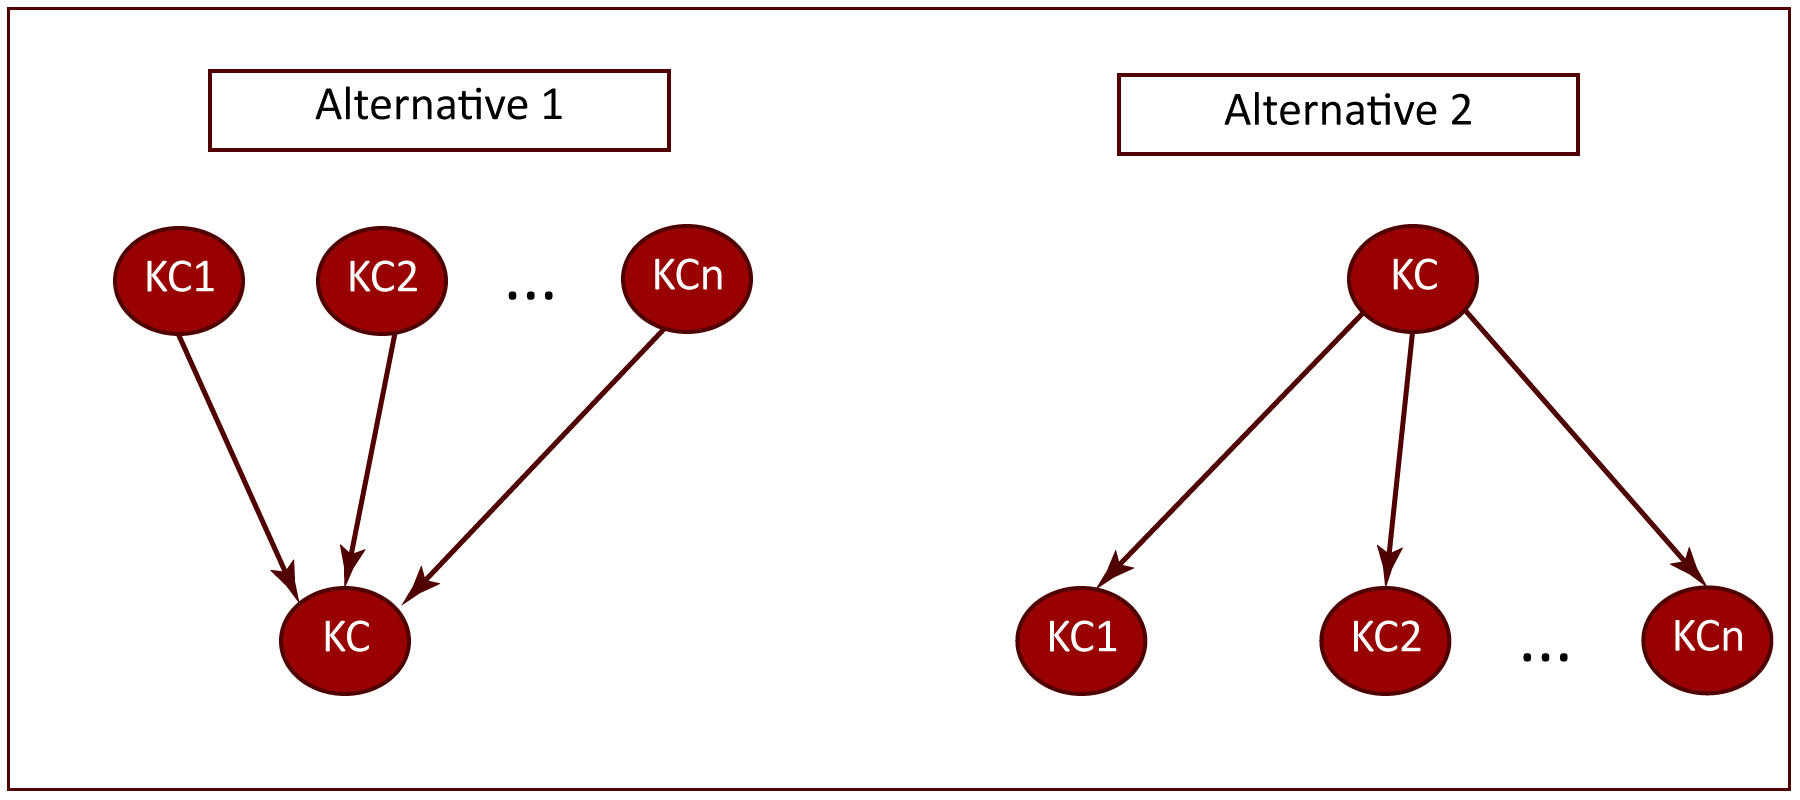
\includegraphics[width=\textwidth]{images/chapitre2/Modèles-d'équations-structurelles.png}
	\end{center}
\caption{Deux alternatives pour modéliser les relations d'agrégation.}
\label{two_agregationrelationships}
\end{figure}

Tchétagni et Nkambou ont proposé d’évaluer les connaissances des apprenants en logique propositionnelle à plusieurs niveaux de granularité. Ils ont utilisé le modèle alternatif 2 de la figure \ref{two_agregationrelationships} pour représenter les relations d'agrégation dans leur hiérarchie. Ils ont souligné que dans cette architecture, il existe des restrictions sur la façon dont les preuves se propagent dans tout le réseau. Cela est dû au fait que deux nœuds enfants peuvent influencer leur parent, sans s'influencer mutuellement : ils sont séparés \cite{hierarchical_representation_evaluation_of_Student_in_ITS}. \\
Carmona et Conejo ont utilisé dans la figure \ref{two_agregationrelationships} le modèle alternatif 1 pour représenter les relations d'agrégation dans leur modèle d'apprenant utilisé dans MEDEA, un système ouvert pour le développement de systèmes de tuteurs intelligents. Certaines approches récentes ont abordé la granularité du modèle de compétences d'un point de vue statistique. 

Dans ces approches, les modèles de compétences n'impliquent que les éléments de connaissance les plus fins, qui expliquent directement les comportements des apprenants. Un problème permanent dans un modèle d’apprenant est de savoir à quel niveau de granularité les compétences des apprenants doivent être modélisées \cite{learner_model_in_distributed_environment}. Pardos et Heffernan ont exploré des modèles avec différents niveaux de granularité (modèles de compétences 1, 5, 39 et 106) et mesuré la précision de ces modèles en prédisant la performance des apprenants dans leur SIT, c'est-à-dire ASSISTment, ainsi que dans un test. Leurs résultats ont montré que plus la granularité du modèle de compétence est fine, meilleure est la prédiction des performances de l'apprenant \cite{Effect_Model_Granularity_on_Student_Performance_Prediction_Using_Bayesian_Networks}.

\subsection{Relations pré-requises}
Des relations préalables existent généralement entre les éléments de connaissance de certains domaines. \\
Reye a analysé comment utiliser les réseaux bayésiens pour modéliser les relations antérieures. Ils ont déclaré que les probabilités conditionnelles dans un réseau bayésien devraient remplir certaines conditions. Par exemple, si la composante de connaissance A est une condition préalable de la composante de connaissance B, l'équation II.1 doit être satisfaite. Cependant, ils ont également déclaré que la relation préalable n'est pas toujours stricte, de sorte qu'ils permettent une incertitude pour les probabilités conditionnelles. Les valeurs d'incertitude pour ces probabilités conditionnelles sont spécifiées par des experts dans leur méthode \cite{Student_Modelling_Based_on_Belief_Networks}.
\begin{equation}
	\begin{split}
		P(learnerKnows(A) \vee  learnerKnows(B)) = 1\\
	P(learnerKnows(B) \vee learnerKnows(A)) = 0
	\end{split}
\end{equation}
Carmona et al. ont présenté les relations préalables à un modèle générique d'apprentissage du BN pour MEDEA, afin d'améliorer l'efficacité des mécanismes d'adaptation et le processus d'inférence. Ils ont utilisé une porte ET bruyante modifiée ou une porte OU bruyante modifiée pour modéliser les relations de prédicat \cite{Prerequisite_Relations_in_Multilayered_Bayesian_Student_Model}. \\
Ferguson et al ont utilisé l'algorithme EM pour apprendre les paramètres cachés dans les BN et ont comparé le modèle de compétence plat (les compétences sont mutuellement indépendantes) avec le modèle de compétence hiérarchique (relations a priori entre des compétences données a priori) selon le critère d'information bayésien (BIC). Leurs résultats montrent qu'un modèle hiérarchique correspond mieux à leurs données que le modèle plat. [20==> a chercher]

\begin{figure}[H]
	\begin{center}
		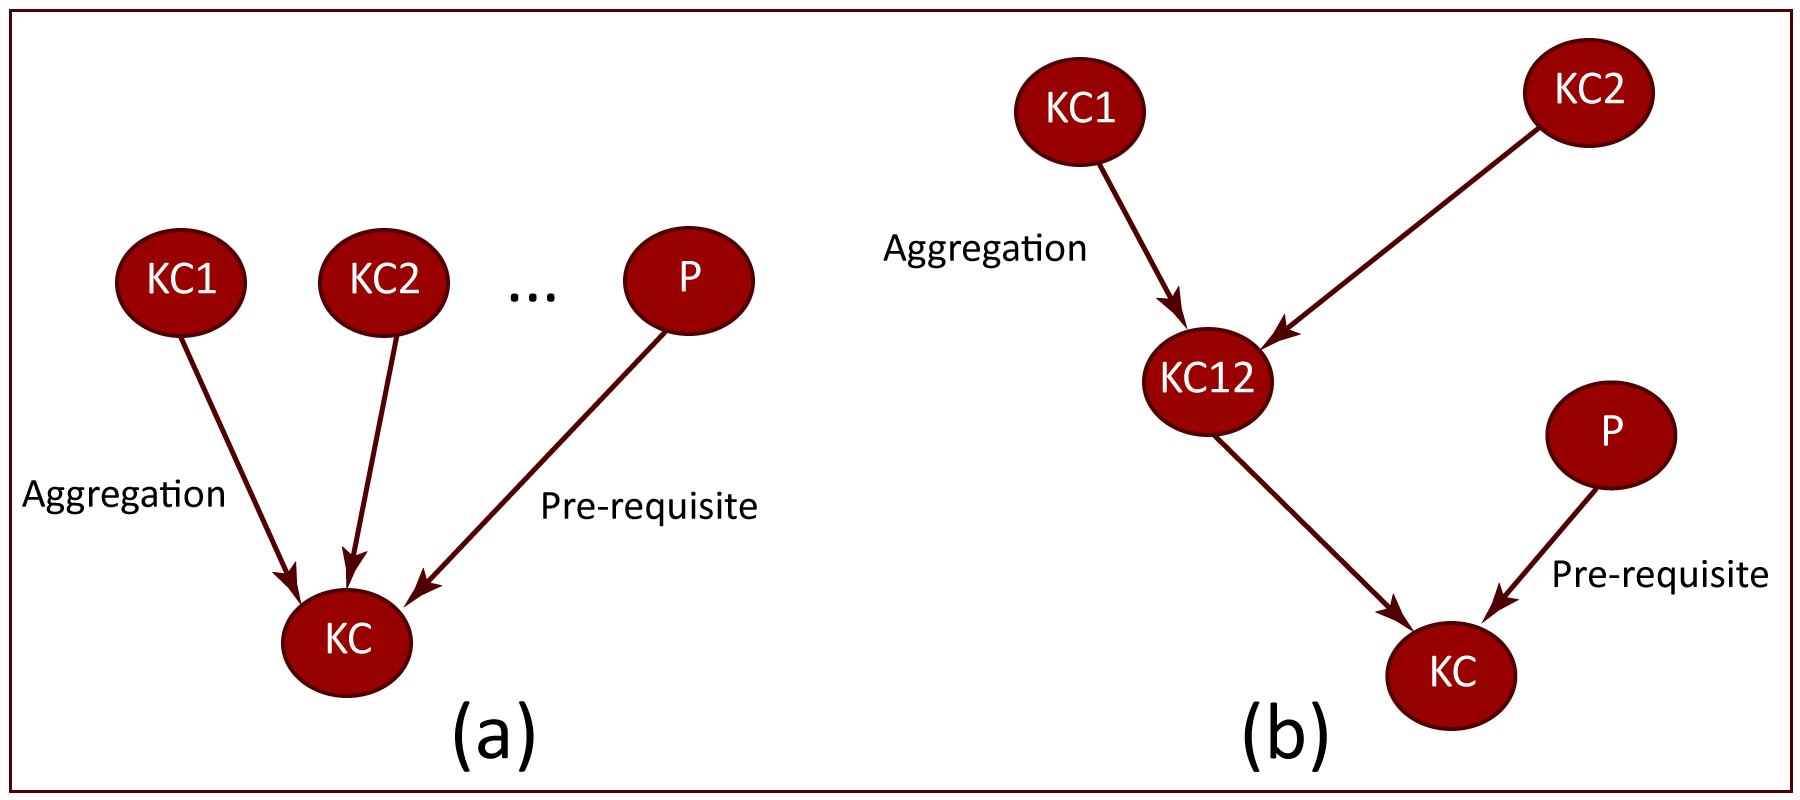
\includegraphics[width=\textwidth]{images/chapitre2/bayesian_network_modeling_aggregationai.png}
	\end{center}
\caption{Agrégation de modélisation de réseau bayésien et relations préalables simultanément}
\label{agregationModelisation}
\end{figure}

Millan et coll. discuté d'un problème courant dans la modélisation des apprenants, à savoir modéliser simultanément les relations de pré-requis et de granularité. Si les deux sont inclus dans le même modèle, les relations avec des interprétations différentes sont mélangées et il est alors difficile de construire et de comprendre le modèle. Par exemple, si une compétence KC composite est composée de deux sous-compétences, KC1 et KC2, il existe également une compétence P qui est un prérequis pour KC. Les probabilités conditionnelles de K données à ses parents sont difficiles à préciser (figure 1.3 (a)). Ils ont proposé une solution qui consiste à regrouper des variables de même type en introduisant des variables intermédiaires (figure 1.3 (b)) \cite{bayesian_networks_student_model_engineering}.

\section{Découverte des prérequis}
Nous modélisons les compétences comme des variables continues qui représentent le degré auquel un apprenant a maîtrisé ou est conscient d'une compétence particulière. Nous traitons les éléments comme des variables continues qui reflètent le degré auquel un apprenant a correctement terminé une tâche. En pratique, la mesure de l'achèvement des tâches est souvent une variable binaire avec des valeurs = correct / incorrect. Un élément binaire peut cependant être considéré comme une projection d'un élément continu, et les corrélations entre éléments continus idéalisés peuvent être estimées en calculant la matrice de corrélation tétrachorique parmi les éléments binaires mesurés \cite{Discovering_Prerequisite_Relationships_among_Knowledge_Components}.

\begin{figure}[H]
	\begin{center}
		\includegraphics[width=\textwidth]{images/chapitre2/modèle_equation_structurelles.png}
	\end{center}
\caption{Modèles d'équations structurelles}
\label{modeleEquation}
\end{figure}

L'utilisation de la matrice Q consiste généralement à définir quels éléments « chargent » sur quelles compétences latentes. Nous pouvons définir un « modèle de mesure » qui relie les compétences latentes aux items mesurés \ref{modeleEquation}. En modélisant les relations entre les compétences comme un modèle analytique causal du chemin entre les variables latentes \ref{modeleEquation}, appelé « modèle structurel », nous pouvons combiner le « modèle de mesure » et le « modèle structurel » pour former un modèle d'équation structurelle linéaire complet \ref{modeleEquation} \cite{Structural_Equations_with_Latent_Variables}. \\
En supposant que le modèle de mesure est connu, nous pouvons rechercher le modèle structurel avec l'algorithme de découverte causale PC, dans lequel les entrées sont les relations d'indépendance et d'indépendance conditionnelle qui figurent parmi les variables latentes. Nous calculons ou testons les relations d'indépendance entre les latents en construisant un modèle structurel séparé et en l'ajustant aux données pour chaque test d'indépendance particulière requis. Notre méthode de construction de modèle produit un test cohérent et éprouvé de chaque relation d'indépendance conditionnelle \cite{Discovering_Prerequisite_Relationships_among_Knowledge_Components}.

\section{Conclusion}
Tout au long de ce chapitre, nous avons présenté les principaux concepts liés au modèle de l'apprenant dans l'environnement de l'apprentissage basé sur le Web, qui permet aux apprenants de travailler en collaboration sur un projet ou de coconstruire le sens des concepts en utilisant la technologie comme un tuyau pour le développement des connaissances partagées, aussi, la modélisation des compétences est importante pour découvrir les prérequis d'un apprenant en représentant le degré auquel il a maîtrisé.
Le prochain chapitre sera consacré à la présentation de l'exploration de données éducatives.








